\begin{figure}[ht]
\label{plot2}
    \centering
    \begin{subfigure}[b]{0.3\textwidth}
        \centering
        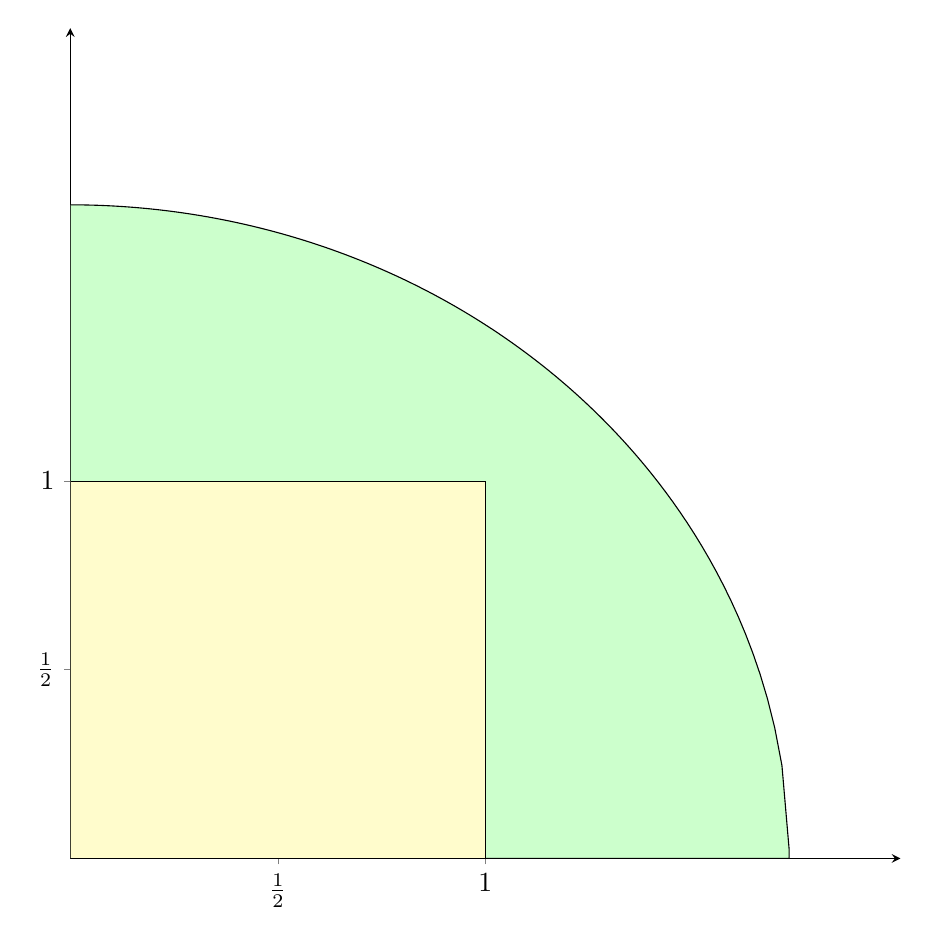
\begin{tikzpicture}
            \begin{axis}[axis lines=middle, 
            xmin=0, xmax=2, 
            ymin=0, ymax=2.2, 
            width=\textwidth, height=\textwidth,
            xtick={0,0.5,1}, % Adjust x-axis ticks
            xticklabels={0,$\frac{1}{2}$,1}, % Custom x-axis labels
            ytick={0.5,1}, % Adjust y-axis ticks
            yticklabels={$ \frac{1}{2}$,1} % Custom y-axis labels 
            ]
                % Quarter circle
                \addplot[domain=0:1.732, samples=100, fill=green!20] {sqrt(3-x^2)} \closedcycle;
                % First cube
                \addplot[fill=yellow!20] coordinates {(0,0) (1,0) (1,1) (0,1) (0,0)};
                % Second cube
                
            \end{axis}
        \end{tikzpicture}
        \caption{collection $C_{1}$}
    \end{subfigure}
    \hfill
    \begin{subfigure}[b]{0.3\textwidth}
        \centering
        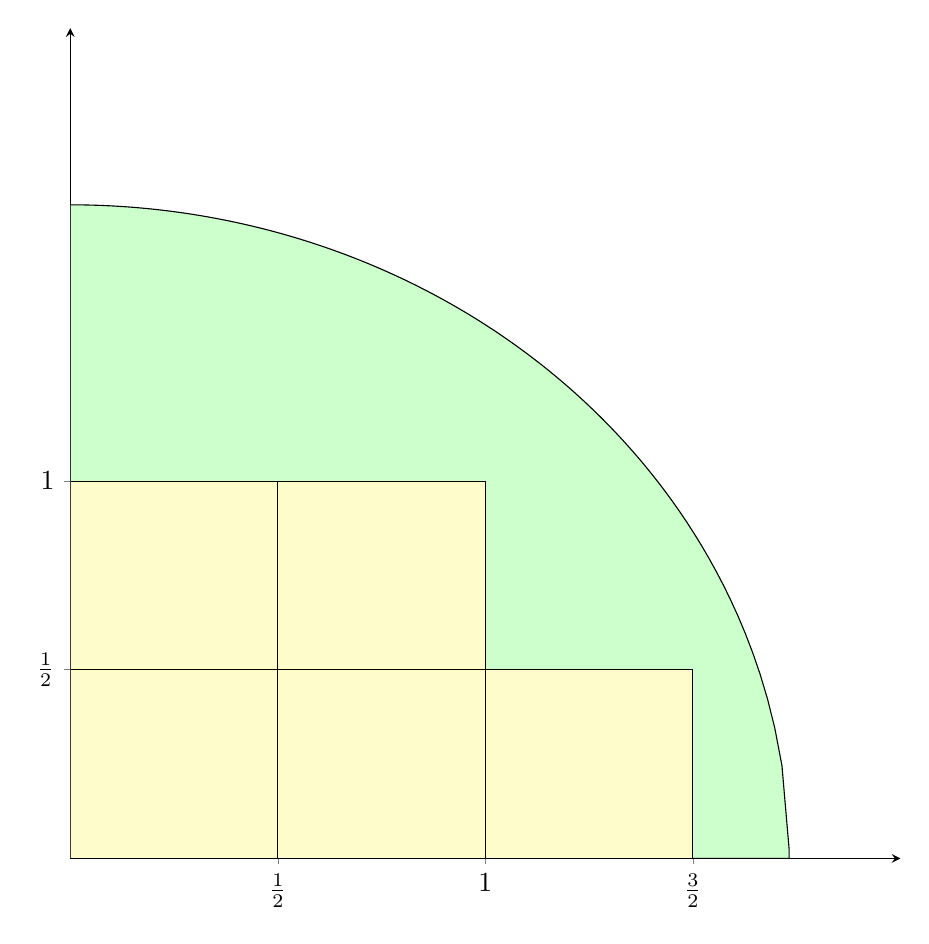
\begin{tikzpicture}
            \begin{axis}[axis lines=middle, 
            xmin=0, xmax=2, 
            ymin=0, ymax=2.2, 
            width=\textwidth, height=\textwidth,
            xtick={0,0.5,1,1.5}, % Adjust x-axis ticks
            xticklabels={0,$\frac{1}{2}$,1,$\frac{3}{2}$}, % Custom x-axis labels
            ytick={0.5,1}, % Adjust y-axis ticks
            yticklabels={$ \frac{1}{2}$,1} % Custom y-axis labels 
            ]
                % Quarter circle
                \addplot[domain=0:1.732, samples=100, fill=green!20] {sqrt(3-x^2)} \closedcycle;
                % Finer cubes
                \addplot[fill=yellow!20] coordinates {(0,0) (0.5,0) (0.5,0.5) (0,0.5) (0,0)};
                \addplot[fill=yellow!20] coordinates {(0.5,0) (1,0) (1,0.5) (0.5,0.5) (0.5,0)};
                \addplot[fill=yellow!20] coordinates {(0,0.5) (0.5,0.5) (0.5,1) (0,1) (0,0.5)};
                \addplot[fill=yellow!20] coordinates {(0.5,0.5) (1,0.5) (1,1) (0.5,1) (0.5,0.5)};
                \addplot[fill=yellow!20] coordinates {(1,0) (1.5,0) (1.5,0.5) (1,0.5) (1,0)};
            \end{axis}
        \end{tikzpicture}
        \caption{collection $C_{2}$}
    \end{subfigure}
    \hfill
    \begin{subfigure}[b]{0.3\textwidth}
        \centering
        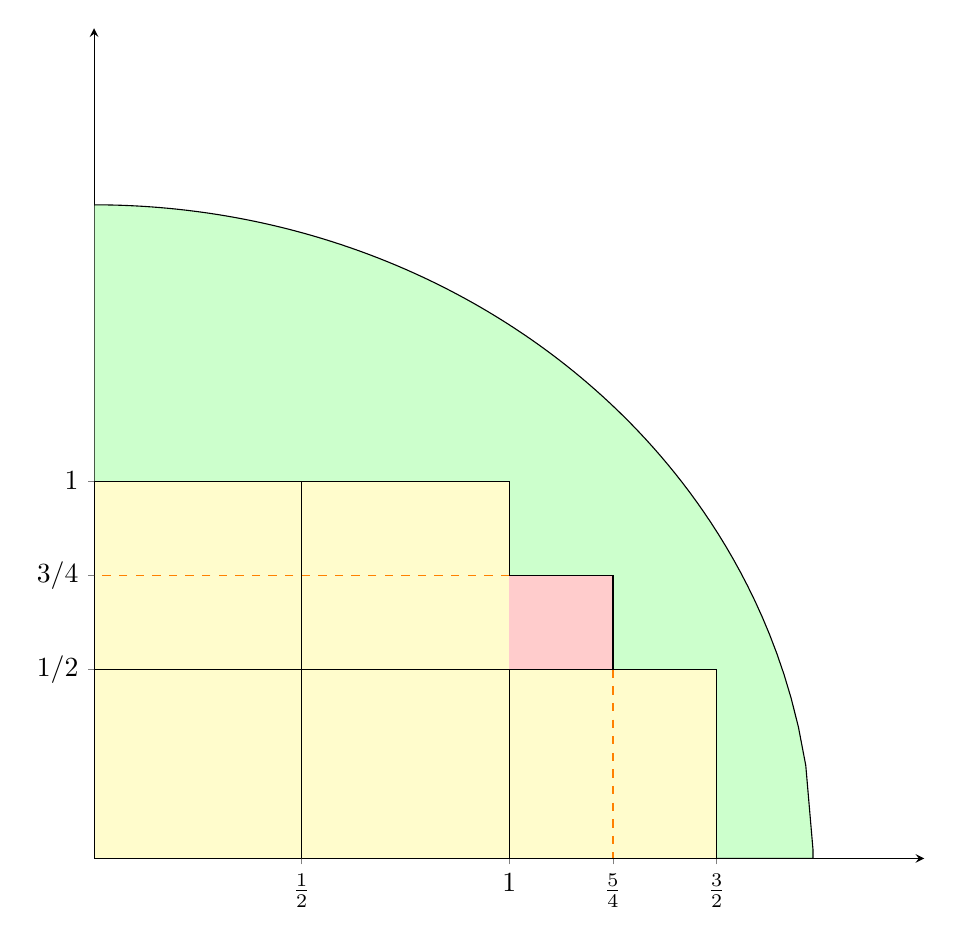
\begin{tikzpicture}
            \begin{axis}[axis lines=middle, 
            xmin=0, xmax=2, 
            ymin=0, ymax=2.2, 
            width=\textwidth, height=\textwidth,
            xtick={0,0.5,1, 1.25, 1.5}, % Adjust x-axis ticks
            xticklabels={0,$\frac{1}{2}$,1, $\frac{5}{4}$, $\frac{3}{2}$}, % Custom x-axis labels
            ytick={0.5, 0.75, 1}, % Adjust y-axis ticks
            yticklabels={$ 1/2$,$3/4$, 1} % Custom y-axis labels 
            ]
                % Quarter circle
                \addplot[domain=0:1.732, samples=100, fill=green!20] {sqrt(3-x^2)} \closedcycle;
                % Finer cubes
                \addplot[fill=yellow!20] coordinates {(0,0) (0.5,0) (0.5,0.5) (0,0.5) (0,0)};
                \addplot[fill=yellow!20] coordinates {(0.5,0) (1,0) (1,0.5) (0.5,0.5) (0.5,0)};
                \addplot[fill=yellow!20] coordinates {(0,0.5) (0.5,0.5) (0.5,1) (0,1) (0,0.5)};
                \addplot[fill=yellow!20] coordinates {(0.5,0.5) (1,0.5) (1,1) (0.5,1) (0.5,0.5)};
                \addplot[fill=yellow!20] coordinates {(1,0) (1.5,0) (1.5,0.5) (1,0.5) (1,0)};
                % Additional cube
                \addplot[fill=red!20] coordinates {(1,0.5) (1.25,0.5) (1.25,0.75) (1,0.75)};
                \addplot[orange, dashed] coordinates {(1.25, 0.5) (1.25, 0)};
                \addplot[orange, dashed] coordinates {(1, 0.75) (0, 0.75)};
            \end{axis}
        \end{tikzpicture}
        \caption{collection $C_3$}
    \end{subfigure}
    \caption{We use dyadic square to approximate the quarter. Note that the sub-collection is not unique since we can choose 4 smaller quads in place of 1-by-1 quad. This process can be viewed as 2D-version of determining series $\{a_{n}\}\in \mathbb{Z}^{n}$ such that $x=\sum a_{n}/2^{n}$ for any real number $x$.}
\end{figure}